\documentclass{article}
\usepackage[utf8]{inputenc}
\usepackage[top=1in]{geometry}
\usepackage{graphicx}
\usepackage{booktabs}
\usepackage{amsmath}
\usepackage{amsthm}
\usepackage[only]{excludeonly}
\usepackage{tikz}
\usetikzlibrary{circuits.logic.US,positioning,calc} 
\usepackage[american]{circuitikz}

% https://tex.stackexchange.com/questions/140567/drawing-karnaughs-maps-in-latex
\usepackage{tikz}
\usetikzlibrary{matrix,calc}

%isolated term
%#1 - Optional. Space between node and grouping line. Default=0
%#2 - node
%#3 - filling color
\newcommand{\implicantsol}[3][0]{
    \draw[rounded corners=3pt, fill=#3, opacity=0.3] ($(#2.north west)+(135:#1)$) rectangle ($(#2.south east)+(-45:#1)$);
    }


%internal group
%#1 - Optional. Space between node and grouping line. Default=0
%#2 - top left node
%#3 - bottom right node
%#4 - filling color
\newcommand{\implicant}[4][0]{
    \draw[rounded corners=3pt, fill=#4, opacity=0.3] ($(#2.north west)+(135:#1)$) rectangle ($(#3.south east)+(-45:#1)$);
    }

%group lateral borders
%#1 - Optional. Space between node and grouping line. Default=0
%#2 - top left node
%#3 - bottom right node
%#4 - filling color
\newcommand{\implicantcostats}[4][0]{
    \draw[rounded corners=3pt, fill=#4, opacity=0.3] ($(rf.east |- #2.north)+(90:#1)$)-| ($(#2.east)+(0:#1)$) |- ($(rf.east |- #3.south)+(-90:#1)$);
    \draw[rounded corners=3pt, fill=#4, opacity=0.3] ($(cf.west |- #2.north)+(90:#1)$) -| ($(#3.west)+(180:#1)$) |- ($(cf.west |- #3.south)+(-90:#1)$);
}

%group top-bottom borders
%#1 - Optional. Space between node and grouping line. Default=0
%#2 - top left node
%#3 - bottom right node
%#4 - filling color
\newcommand{\implicantdaltbaix}[4][0]{
    \draw[rounded corners=3pt, fill=#4, opacity=0.3] ($(cf.south -| #2.west)+(180:#1)$) |- ($(#2.south)+(-90:#1)$) -| ($(cf.south -| #3.east)+(0:#1)$);
    \draw[rounded corners=3pt, fill=#4, opacity=0.3] ($(rf.north -| #2.west)+(180:#1)$) |- ($(#3.north)+(90:#1)$) -| ($(rf.north -| #3.east)+(0:#1)$);
}

%group corners
%#1 - Optional. Space between node and grouping line. Default=0
%#2 - filling color
\newcommand{\implicantcantons}[2][0]{
    \draw[rounded corners=3pt, opacity=.3] ($(rf.east |- 0.south)+(-90:#1)$) -| ($(0.east |- cf.south)+(0:#1)$);
    \draw[rounded corners=3pt, opacity=.3] ($(rf.east |- 8.north)+(90:#1)$) -| ($(8.east |- rf.north)+(0:#1)$);
    \draw[rounded corners=3pt, opacity=.3] ($(cf.west |- 2.south)+(-90:#1)$) -| ($(2.west |- cf.south)+(180:#1)$);
    \draw[rounded corners=3pt, opacity=.3] ($(cf.west |- 10.north)+(90:#1)$) -| ($(10.west |- rf.north)+(180:#1)$);
    \fill[rounded corners=3pt, fill=#2, opacity=.3] ($(rf.east |- 0.south)+(-90:#1)$) -|  ($(0.east |- cf.south)+(0:#1)$) [sharp corners] ($(rf.east |- 0.south)+(-90:#1)$) |-  ($(0.east |- cf.south)+(0:#1)$) ;
    \fill[rounded corners=3pt, fill=#2, opacity=.3] ($(rf.east |- 8.north)+(90:#1)$) -| ($(8.east |- rf.north)+(0:#1)$) [sharp corners] ($(rf.east |- 8.north)+(90:#1)$) |- ($(8.east |- rf.north)+(0:#1)$) ;
    \fill[rounded corners=3pt, fill=#2, opacity=.3] ($(cf.west |- 2.south)+(-90:#1)$) -| ($(2.west |- cf.south)+(180:#1)$) [sharp corners]($(cf.west |- 2.south)+(-90:#1)$) |- ($(2.west |- cf.south)+(180:#1)$) ;
    \fill[rounded corners=3pt, fill=#2, opacity=.3] ($(cf.west |- 10.north)+(90:#1)$) -| ($(10.west |- rf.north)+(180:#1)$) [sharp corners] ($(cf.west |- 10.north)+(90:#1)$) |- ($(10.west |- rf.north)+(180:#1)$) ;
}

%Empty Karnaugh map 4x4
\newenvironment{Karnaugh}[2]%
{
\begin{tikzpicture}[baseline=(current bounding box.north),scale=0.8]
\draw (0,0) grid (4,4);
\draw (0,4) -- node [pos=0.7,above right,anchor=south west] {#1} node [pos=0.7,below left,anchor=north east] {#2} ++(135:1);
%
\matrix (mapa) [matrix of nodes,
        column sep={0.8cm,between origins},
        row sep={0.8cm,between origins},
        every node/.style={minimum size=0.3mm},
        anchor=2.center,
        ampersand replacement=\&] at (0.5,0.5)
{
                       \& |(c00)| 00         \& |(c01)| 01         \& |(c11)| 11         \& |(c10)| 10         \& |(cf)| \phantom{00} \\
|(r00)| 00             \& |(0)|  \phantom{0} \& |(4)|  \phantom{0} \& |(12)|  \phantom{0} \& |(8)|  \phantom{0} \&                     \\
|(r01)| 01             \& |(1)|  \phantom{0} \& |(5)|  \phantom{0} \& |(13)|  \phantom{0} \& |(9)|  \phantom{0} \&                     \\
|(r11)| 11             \& |(3)| \phantom{0} \& |(7)| \phantom{0} \& |(15)| \phantom{0} \& |(11)| \phantom{0} \&                     \\
|(r10)| 10             \& |(2)|  \phantom{0} \& |(6)|  \phantom{0} \& |(14)| \phantom{0} \& |(10)| \phantom{0} \&                     \\
|(rf) | \phantom{00}   \&                    \&                    \&                    \&                    \&                     \\
};
}%
{
\end{tikzpicture}
}

%Empty Karnaugh map 2x4
\newenvironment{Karnaughvuit}%
{
\begin{tikzpicture}[baseline=(current bounding box.north),scale=0.8]
\draw (0,0) grid (4,2);
\draw (0,2) -- node [pos=0.7,above right,anchor=south west] {AB} node [pos=0.7,below left,anchor=north east] {C} ++(135:1);
%
\matrix (mapa) [matrix of nodes,
        column sep={0.8cm,between origins},
        row sep={0.8cm,between origins},
        every node/.style={minimum size=0.3mm},
        anchor=1.center,
        ampersand replacement=\&] at (0.5,0.5)
{
                      \& |(c00)| 00         \& |(c01)| 01         \& |(c11)| 11         \& |(c10)| 10         \& |(cf)| \phantom{00} \\
|(r00)| 0             \& |(0)|  \phantom{0} \& |(2)|  \phantom{0} \& |(6)|  \phantom{0} \& |(4)|  \phantom{0} \&                     \\
|(r01)| 1             \& |(1)|  \phantom{0} \& |(3)|  \phantom{0} \& |(7)|  \phantom{0} \& |(5)|  \phantom{0} \&                     \\
|(rf) | \phantom{00}  \&                    \&                    \&                    \&                    \&                     \\
};
}%
{
\end{tikzpicture}
}

%Empty Karnaugh map 2x2
\newenvironment{Karnaughquatre}%
{
\begin{tikzpicture}[baseline=(current bounding box.north),scale=0.8]
\draw (0,0) grid (2,2);
\draw (0,2) -- node [pos=0.7,above right,anchor=south west] {A} node [pos=0.7,below left,anchor=north east] {B} ++(135:1);
%
\matrix (mapa) [matrix of nodes,
        column sep={0.8cm,between origins},
        row sep={0.8cm,between origins},
        every node/.style={minimum size=0.3mm},
        anchor=1.center,
        ampersand replacement=\&] at (0.5,0.5)
{
          \& |(c00)| 0          \& |(c01)| 1  \\
|(r00)| 0 \& |(0)|  \phantom{0} \& |(2)|  \phantom{0} \\
|(r01)| 1 \& |(1)|  \phantom{0} \& |(3)|  \phantom{0} \\
};
}%
{
\end{tikzpicture}
}

%Defines 8 or 16 values (0,1,X)
\newcommand{\contingut}[1]{%
\foreach \x [count=\xi from 0]  in {#1}
     \path (\xi) node {\x};
}

%Places 1 in listed positions
\newcommand{\minterms}[1]{%
    \foreach \x in {#1}
        \path (\x) node {1};
}

%Places 0 in listed positions
\newcommand{\maxterms}[1]{%
    \foreach \x in {#1}
        \path (\x) node {0};
}

%Places X in listed positions
\newcommand{\indeterminats}[1]{%
    \foreach \x in {#1}
        \path (\x) node {X};
}

% Places m_{x} in listed positions
\newcommand{\phminterms}[1]{%
  \foreach \x in {#1}
  \path (\x) node {$m_{\x}$};
}

% Places m_{16+x} in listed positions
\newcommand{\phmintermssixt}[1]{%
  \foreach [evaluate={\y=int(16+\x)}] \x in {#1}
  \path (\x) node {$m_{\y}$};
}

% Calligraphic fonts
\newcommand{\calA}{{\cal A}}
\newcommand{\calB}{{\cal B}}
\newcommand{\calC}{{\cal C}}
\newcommand{\calD}{{\cal D}}
\newcommand{\calE}{{\cal E}}
\newcommand{\calF}{{\cal F}}
\newcommand{\calG}{{\cal G}}
\newcommand{\calH}{{\cal H}}
\newcommand{\calI}{{\cal I}}
\newcommand{\calJ}{{\cal J}}
\newcommand{\calK}{{\cal K}}
\newcommand{\calL}{{\cal L}}
\newcommand{\calM}{{\cal M}}
\newcommand{\calN}{{\cal N}}
\newcommand{\calO}{{\cal O}}
\newcommand{\calP}{{\cal P}}
\newcommand{\calQ}{{\cal Q}}
\newcommand{\calR}{{\cal R}}
\newcommand{\calS}{{\cal S}}
\newcommand{\calT}{{\cal T}}
\newcommand{\calU}{{\cal U}}
\newcommand{\calV}{{\cal V}}
\newcommand{\calW}{{\cal W}}
\newcommand{\calX}{{\cal X}}
\newcommand{\calY}{{\cal Y}}
\newcommand{\calZ}{{\cal Z}}

% Sets:
\newcommand{\setA}{\textsf{A}}
\newcommand{\setB}{\textsf{B}}
\newcommand{\setC}{\textsf{C}}
\newcommand{\setD}{\textsf{D}}
\newcommand{\setE}{\textsf{E}}
\newcommand{\setF}{\textsf{F}}
\newcommand{\setG}{\textsf{G}}
\newcommand{\setH}{\textsf{H}}
\newcommand{\setI}{\textsf{I}}
\newcommand{\setJ}{\textsf{J}}
\newcommand{\setK}{\textsf{K}}
\newcommand{\setL}{\textsf{L}}
\newcommand{\setM}{\textsf{M}}
\newcommand{\setN}{\textsf{N}}
\newcommand{\setO}{\textsf{O}}
\newcommand{\setP}{\textsf{P}}
\newcommand{\setQ}{\textsf{Q}}
\newcommand{\setR}{\textsf{R}}
\newcommand{\setS}{\textsf{S}}
\newcommand{\setT}{\textsf{T}}
\newcommand{\setU}{\textsf{U}}
\newcommand{\setV}{\textsf{V}}
\newcommand{\setW}{\textsf{W}}
\newcommand{\setX}{\textsf{X}}
\newcommand{\setY}{\textsf{Y}}
\newcommand{\setZ}{\textsf{Z}}

% Vectors
\newcommand{\bfa}{\mathbf{a}}
\newcommand{\bfb}{\mathbf{b}}
\newcommand{\bfc}{\mathbf{c}}
\newcommand{\bfd}{\mathbf{d}}
\newcommand{\bfe}{\mathbf{e}}
\newcommand{\bff}{\mathbf{f}}
\newcommand{\bfg}{\mathbf{g}}
\newcommand{\bfh}{\mathbf{h}}
\newcommand{\bfi}{\mathbf{i}}
\newcommand{\bfj}{\mathbf{j}}
\newcommand{\bfk}{\mathbf{k}}
\newcommand{\bfl}{\mathbf{l}}
\newcommand{\bfm}{\mathbf{m}}
\newcommand{\bfn}{\mathbf{n}}
\newcommand{\bfo}{\mathbf{o}}
\newcommand{\bfp}{\mathbf{p}}
\newcommand{\bfq}{\mathbf{q}}
\newcommand{\bfr}{\mathbf{r}}
\newcommand{\bfs}{\mathbf{s}}
\newcommand{\bft}{\mathbf{t}}
\newcommand{\bfu}{\mathbf{u}}
\newcommand{\bfv}{\mathbf{v}}
\newcommand{\bfw}{\mathbf{w}}
\newcommand{\bfx}{\mathbf{x}}
\newcommand{\bfy}{\mathbf{y}}
\newcommand{\bfz}{\mathbf{z}}


\newcommand{\bfalpha}{\boldsymbol{\alpha}}
\newcommand{\bfbeta}{\boldsymbol{\beta}}
\newcommand{\bfgamma}{\boldsymbol{\gamma}}
\newcommand{\bfdelta}{\boldsymbol{\delta}}
\newcommand{\bfepsilon}{\boldsymbol{\epsilon}}
\newcommand{\bfzeta}{\boldsymbol{\zeta}}
\newcommand{\bfeta}{\boldsymbol{\eta}}
\newcommand{\bftheta}{\boldsymbol{\theta}}
\newcommand{\bfiota}{\boldsymbol{\iota}}
\newcommand{\bfkappa}{\boldsymbol{\kappa}}
\newcommand{\bflambda}{\boldsymbol{\lambda}}
\newcommand{\bfmu}{\boldsymbol{\mu}}
\newcommand{\bfnu}{\boldsymbol{\nu}}
\newcommand{\bfomicron}{\boldsymbol{\omicron}}
\newcommand{\bfpi}{\boldsymbol{\pi}}
\newcommand{\bfrho}{\boldsymbol{\rho}}
\newcommand{\bfsigma}{\boldsymbol{\sigma}}
\newcommand{\bftau}{\boldsymbol{\tau}}
\newcommand{\bfupsilon}{\boldsymbol{\upsilon}}
\newcommand{\bfphi}{\boldsymbol{\phi}}
\newcommand{\bfchi}{\boldsymbol{\chi}}
\newcommand{\bfpsi}{\boldsymbol{\psi}}
\newcommand{\bfomega}{\boldsymbol{\omega}}
\newcommand{\bfxi}{\boldsymbol{\xi}}
\newcommand{\bfell}{\boldsymbol{\ell}}

% Matrices
\newcommand{\bfA}{\mathbf{A}}
\newcommand{\bfB}{\mathbf{B}}
\newcommand{\bfC}{\mathbf{C}}
\newcommand{\bfD}{\mathbf{D}}
\newcommand{\bfE}{\mathbf{E}}
\newcommand{\bfF}{\mathbf{F}}
\newcommand{\bfG}{\mathbf{G}}
\newcommand{\bfH}{\mathbf{H}}
\newcommand{\bfI}{\mathbf{I}}
\newcommand{\bfJ}{\mathbf{J}}
\newcommand{\bfK}{\mathbf{K}}
\newcommand{\bfL}{\mathbf{L}}
\newcommand{\bfM}{\mathbf{M}}
\newcommand{\bfN}{\mathbf{N}}
\newcommand{\bfO}{\mathbf{O}}
\newcommand{\bfP}{\mathbf{P}}
\newcommand{\bfQ}{\mathbf{Q}}
\newcommand{\bfR}{\mathbf{R}}
\newcommand{\bfS}{\mathbf{S}}
\newcommand{\bfT}{\mathbf{T}}
\newcommand{\bfU}{\mathbf{U}}
\newcommand{\bfV}{\mathbf{V}}
\newcommand{\bfW}{\mathbf{W}}
\newcommand{\bfX}{\mathbf{X}}
\newcommand{\bfY}{\mathbf{Y}}
\newcommand{\bfZ}{\mathbf{Z}}


\newcommand{\bfGamma}{\boldsymbol{\Gamma}}
\newcommand{\bfDelta}{\boldsymbol{\Delta}}
\newcommand{\bfTheta}{\boldsymbol{\Theta}}
\newcommand{\bfLambda}{\boldsymbol{\Lambda}}
\newcommand{\bfPi}{\boldsymbol{\Pi}}
\newcommand{\bfSigma}{\boldsymbol{\Sigma}}
\newcommand{\bfUpsilon}{\boldsymbol{\Upsilon}}
\newcommand{\bfPhi}{\boldsymbol{\Phi}}
\newcommand{\bfPsi}{\boldsymbol{\Psi}}
\newcommand{\bfOmega}{\boldsymbol{\Omega}}


% Blackboard Bold:
\newcommand{\bbA}{\mathbb{A}}
\newcommand{\bbB}{\mathbb{B}}
\newcommand{\bbC}{\mathbb{C}}
\newcommand{\bbD}{\mathbb{D}}
\newcommand{\bbE}{\mathbb{E}}
\newcommand{\bbF}{\mathbb{F}}
\newcommand{\bbG}{\mathbb{G}}
\newcommand{\bbH}{\mathbb{H}}
\newcommand{\bbI}{\mathbb{I}}
\newcommand{\bbJ}{\mathbb{J}}
\newcommand{\bbK}{\mathbb{K}}
\newcommand{\bbL}{\mathbb{L}}
\newcommand{\bbM}{\mathbb{M}}
\newcommand{\bbN}{\mathbb{N}}
\newcommand{\bbO}{\mathbb{O}}
\newcommand{\bbP}{\mathbb{P}}
\newcommand{\bbQ}{\mathbb{Q}}
\newcommand{\bbR}{\mathbb{R}}
\newcommand{\bbS}{\mathbb{S}}
\newcommand{\bbT}{\mathbb{T}}
\newcommand{\bbU}{\mathbb{U}}
\newcommand{\bbV}{\mathbb{V}}
\newcommand{\bbW}{\mathbb{W}}
\newcommand{\bbX}{\mathbb{X}}
\newcommand{\bbY}{\mathbb{Y}}
\newcommand{\bbZ}{\mathbb{Z}}




\author{Vikas Dhiman for ECE275}
\newtheorem{example}{Example}
\newtheorem{prob}{Problem}
\newtheorem{remark}{Remark}
\newtheorem{definition}{Definition}

\newcommand{\bx}{\bar{x}}
\newcommand{\by}{\bar{y}}
\newcommand{\bz}{\bar{z}}
\newcommand{\bA}{\bar{A}}
\newcommand{\bB}{\bar{B}}
\newcommand{\bC}{\bar{C}}
\newcommand{\bD}{\bar{D}}

\newcommand{\notescol}{white}
\title{Analog details behind the digital abstraction}
\begin{document}

\maketitle

Some of the material is out of the textbook. Additional resources include
Appendix B of Brown and Vranesic book, ``Fundamentals of digital logic.''

\section{Objectives}
\begin{enumerate}
\item Describe how tri-state and open-collector outputs are different from totem-pole outputs
\item Compute noise margin of one device driving the same time
\item Understand timing diagrams, gate delays and critical path
\item Design Hazard-free two level circuits
\end{enumerate}

\section{Logic levels and Noise Margins}

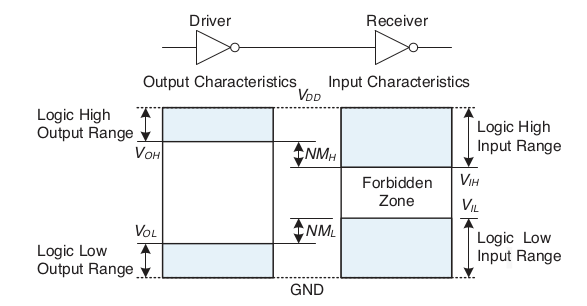
\includegraphics[width=0.8\linewidth]{fig/logic-levels-and-noise-margins.png}

\begin{definition}[Supply Voltage ($V_{DD}$/$V_{CC}$/$V_{SS}$) ]
  \color{\notescol}
  The highest DC voltage that drives a digital circuit. As chips have progressed
  to smaller transistors, $V_{DD}$ has dropped from 5V to 1.2V or even lower to
  save power.
\end{definition}

\begin{definition}[Ground Voltage ($V_{GND}$) ]
  \color{\notescol}
  The lowest DC voltage that drives a digital circuit, typically 0V.
\end{definition}

\begin{definition}[Input high ($V_{IH}$) and Input Low ($V_{IL}$) of a gate]
  \color{\notescol}
  $V_{IH}$ is the voltage level, such that an input voltage to a gate between $V_{DD}$
  and $V_{IH}$ is considered \emph{HIGH}. Similarly, input voltage to a gate
  between $V_{IL}$ and $V_{GND}$ is considered \emph{LOW}.
\end{definition}

\begin{definition}[Output high ($V_{OH}$) and Output low ($V_{OL}$) of gate]
  \color{\notescol}
  $V_{OH}$ is the voltage level, such that an output voltage to a gate between $V_{DD}$
  and $V_{OH}$ is considered \emph{HIGH}. Similarly, output voltage to a gate
  between $V_{OL}$ and $V_{GND}$ is considered \emph{LOW}.
\end{definition}

\begin{definition}[Positive logic and Negative logic]
  \color{\notescol}
  What we have considered so far is Positive logic where \emph{HIGH} voltage is
  equated to Boolean logic \emph{TRUE} or \emph{1} and \emph{LOW} is considered
  \emph{FALSE} or \emph{0}. In negative logic these are reversed. Same physical
  circuit can represent different logical circuits in positive logic and
  negative logic.
\end{definition}

\begin{definition}[Noise margins ($NM_L$ and $NM_H$) of a channel]
  \color{\notescol}
  The maximum amount of noise that can be added (or substracted ) to a channel
  without exceeding the logic level specifications of a gate.  
  $NM_L  = V_{IL} - V_{OL}$ \\
  $NM_H  = V_{OH} - V_{IH}$
\end{definition}

\begin{example}
  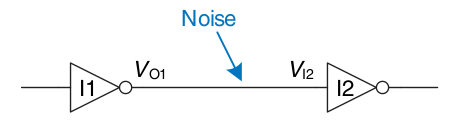
\includegraphics[width=0.3\linewidth]{fig/fig1.24-noise-margins.png}\\
  If $V_{DD} = 5V$ , $V_{IL} = 1.35V$, $V_{IH} = 3.15V$, $V_{OL} = 0.33V$ and
  $V_{OH} = 3.84V$ for both the ``inverters'', then what are the low and high
  noise margins? Can the circuit tolerate 1V of noise at the channel?
\end{example}
\vspace{10em}

\section{Semiconductors and Doping}
{\tiny{Not in syllabus but good to know}}

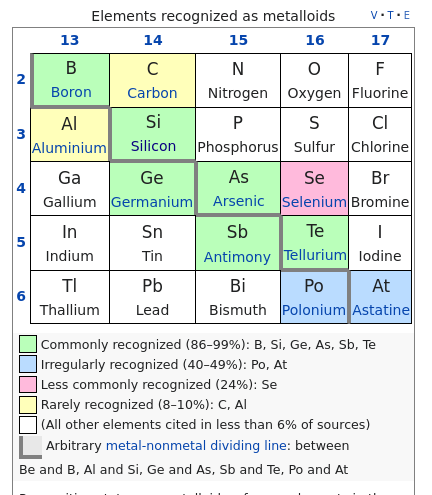
\includegraphics[width=0.5\linewidth]{fig/semiconductors-periodic-table.png}


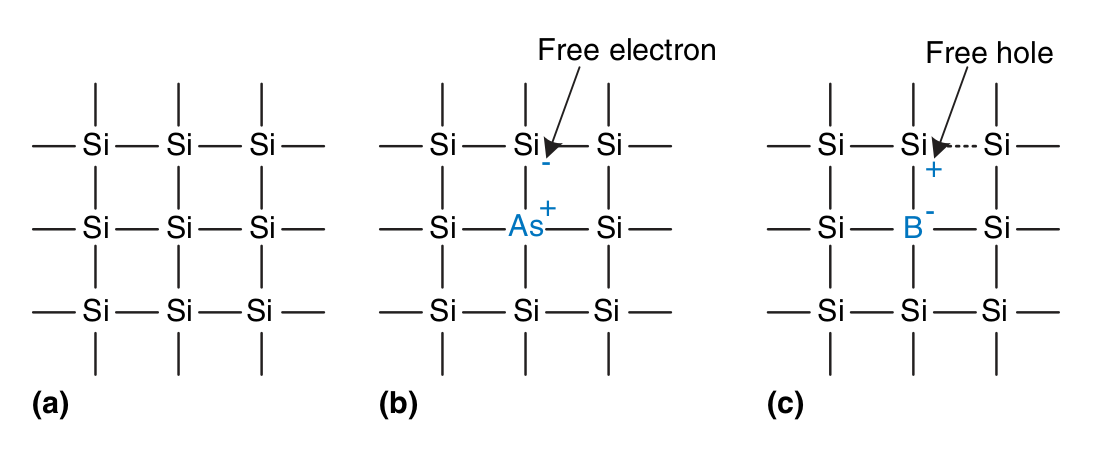
\includegraphics[width=0.8\linewidth]{fig/fig1.26-Si-doping.png}

\section{MOSFET: Metal Oxide Field Effect Transistors }
{\tiny{Not in syllabus but good to know}}

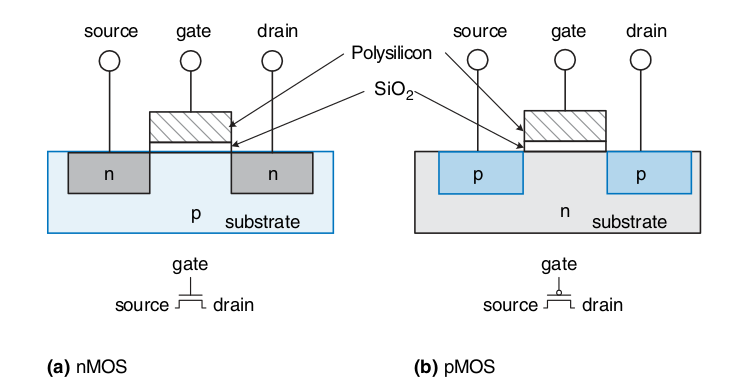
\includegraphics[width=0.8\linewidth]{fig/fig1.29-nMOS-pMOS-transistors.png}

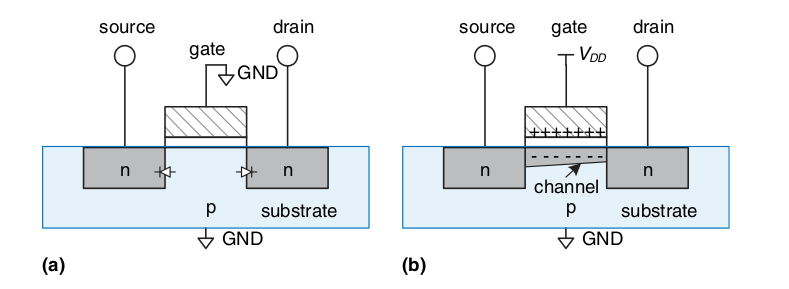
\includegraphics[width=0.8\linewidth]{fig/fig1.30-nMOS-transistor-operation.png}

\section{DC Transfer characteristic}

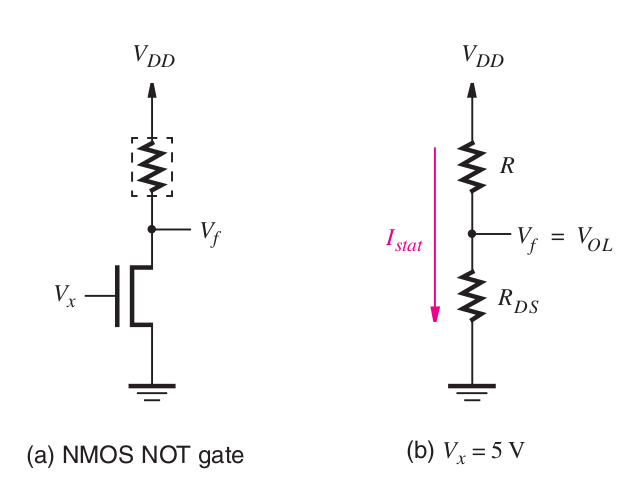
\includegraphics[width=0.6\linewidth]{fig/nMOS-not-gate.png}

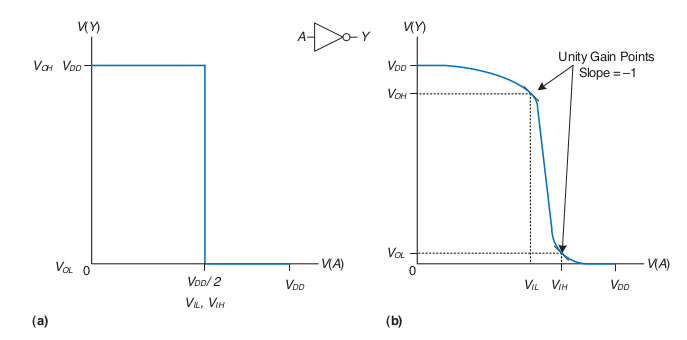
\includegraphics[width=0.8\linewidth]{fig/fig1.25-dc-transfer-characteristics.png}

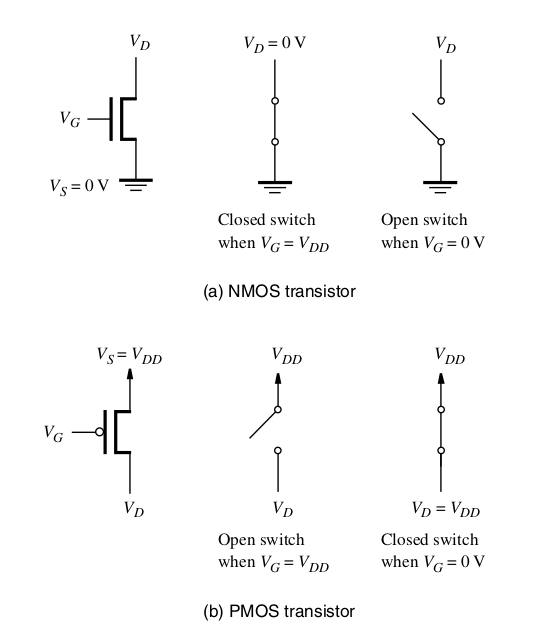
\includegraphics[width=0.7\linewidth]{fig/nMOS-pMOS-switches.png}


\begin{example}
  Draw a NOT gate using nMOS transistors.
\end{example}
\vspace{10em}

\begin{example}
  Draw a NOT gate using pMOS transistors.
\end{example}
\vspace{10em}

\begin{remark}
  nMOS transistors pass 0's well (output between 0 and $V_{DD} - V_t$). pMOS
  transistors pass 1's well (output between $V_t$ and $V_{DD}$).
\end{remark}
\begin{example}
Draw CMOS NOT Gate.
\end{example}
\vspace{10em}

\begin{example}
Draw a two input CMOS NAND Gate
\end{example}
\vspace{10em}


\begin{definition}[Negative logic]
\end{definition}
\vspace{5em}

\begin{example}
  Analyze the above circuit under negative logic.
\end{example}
\vspace{10em}



\begin{example}
Draw a three input NAND using CMOS.
\end{example}
\vspace{10em}


\begin{example}
Draw a three input NOR using CMOS.
\end{example}
\vspace{10em}

\begin{example}
  Draw a two input AND gate using CMOS.
\end{example}
\vspace{10em}

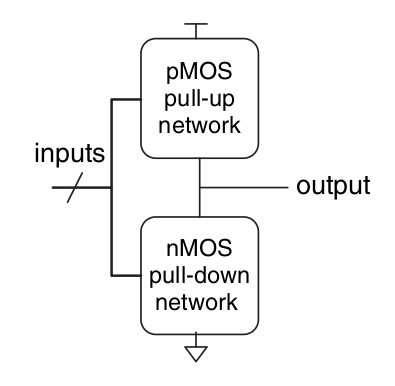
\includegraphics[width=0.4\linewidth]{fig/fig1.34-inverting-logic-gate.png}

\subsection{Gates with floating output}
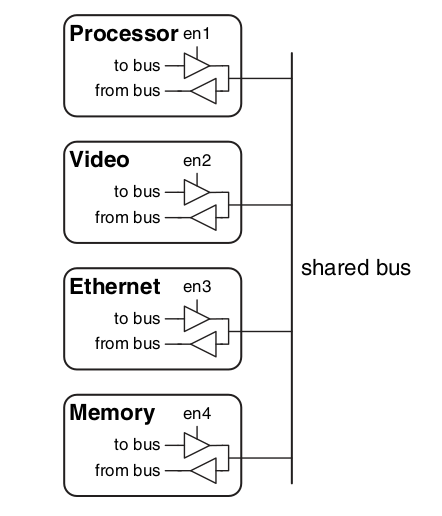
\includegraphics[width=0.4\linewidth]{fig/fig2.42-tristate-bus.png}

\begin{definition}[Transmission gate]
  Draw a schematic of transmission gate and truth table for transmission gate.
  What is its commonly used symbol?
\end{definition}
\vspace{10em}


\begin{definition}[Tristate buffer]
  What is tristate buffer? Draw it's symbol and truth table? Where is it used?
\end{definition}
\vspace{10em}

\begin{example}
Draw a Multiplexer using transmission gates.
\end{example}
\vspace{10em}

\begin{example}
  Draw a Multiplexer using tristate buffers.
\end{example}
\vspace{10em}


\begin{definition}[Totem-pole]
  Draw a Push-pull (or Totem-pole) output NAND gate using CMOS. Can you connect
  this gate to a shared bus?
\end{definition}
\vspace{10em}

\begin{definition}[Tristate]
  Draw a Tristate output NAND gate using CMOS with an output enable (OE) input.
  Can you connect this gate to a shared bus?
\end{definition}
\vspace{10em}

\begin{definition}[Open-collector]
  Draw a open-collector output NAND gate. Can you connect this gate to a shared bus?
\end{definition}
\vspace{10em}

\section{Verilog truth tables}

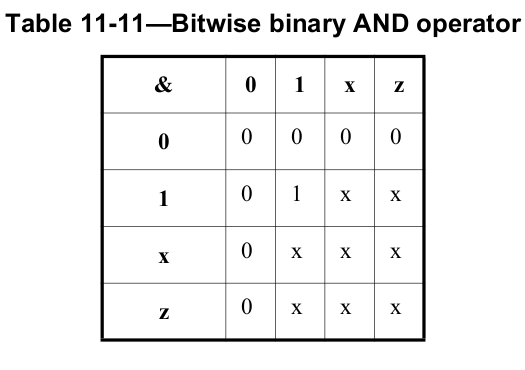
\includegraphics[width=0.3\linewidth]{fig/four-state-and-operator.png}
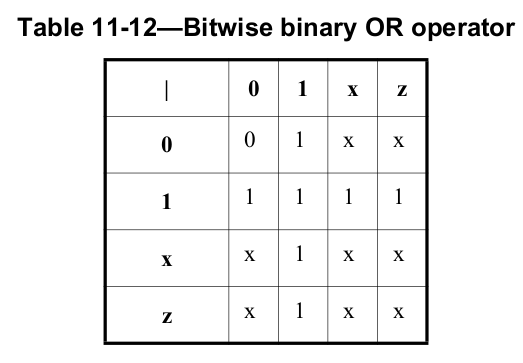
\includegraphics[width=0.3\linewidth]{fig/four-state-or-operator.png}

\section{Timing diagrams and propagation delays}

\begin{example}[Timing diagram]
  Draw a timing diagram for an ideal NAND gate.
\end{example}
\vspace{20em}

\subsection{Delays}
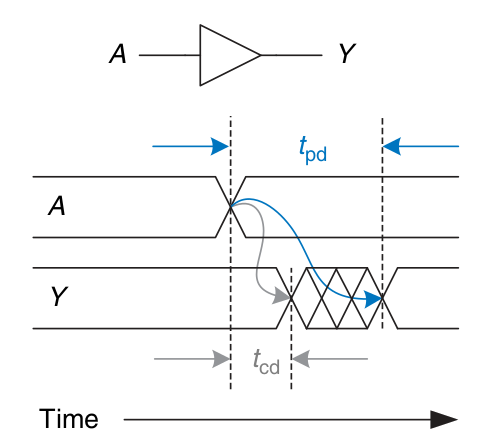
\includegraphics[width=0.5\linewidth]{fig/fig2.67-delays-tpd-tcd.png}
\begin{definition}[Propagation delay ($t_{pd}$)]
\end{definition}
\vspace{5em}

\begin{definition}[Contamination delay ($t_{cd}$)]
\end{definition}
\vspace{5em}

\subsection{Paths}
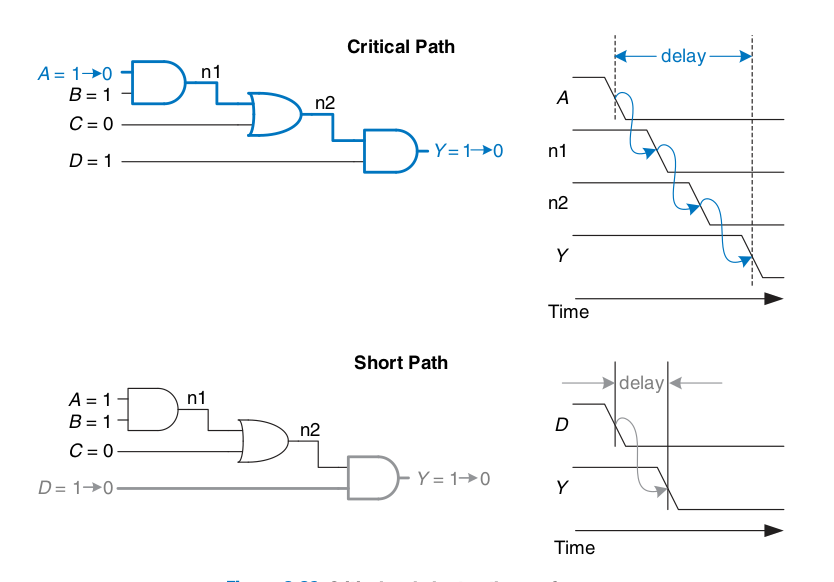
\includegraphics[width=0.8\linewidth]{fig/fig2.68-short-path-and-critical-path.png}
\begin{example}
  Find the propagation delay of the circuit above given that propagation delay
  of each gate is $100 ps$  add contamination delay of $60ps$.
\end{example}
\vspace{10em}

\section{Glitches or Hazards}
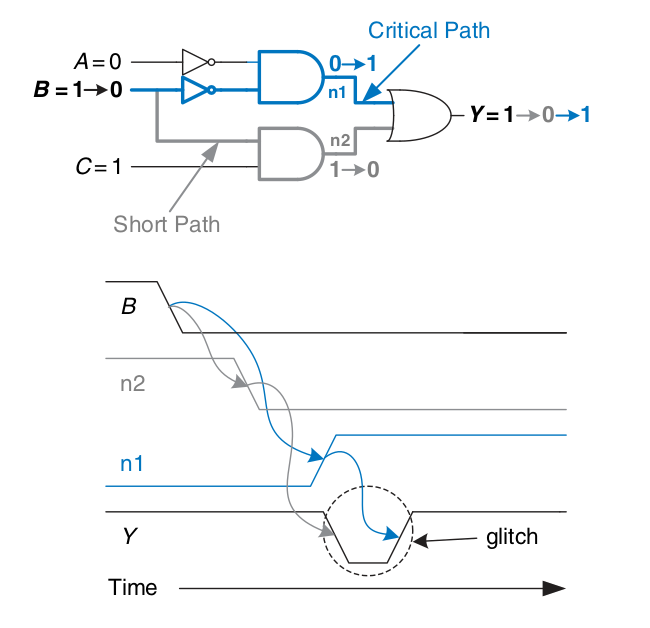
\includegraphics[width=0.6\linewidth]{fig/fig2.76-timing-of-a-glitch.png}
\begin{definition}[Glitch or Hazard]

\end{definition}
\vspace{5em}

\begin{example}
  Design a circuit that fixes the glitch in the above circuit (also known as
  glitch-free or hazard-free circuit).
\end{example}
\vspace{10em}

%\bibliography{main}
%\bibliographystyle{plain}
\end{document}
